\section{O crivo de Erastótenes}

\begin{frame}[fragile]{Listagem dos $N$ primeiros primos}

    \begin{itemize}
        \item Na prática, para se verificar se um ou poucos números são primos,
            \code{cpp}{is_prime3()} é suficiente

        \item Para verificar um conjunto de inteiros $n$, pode ser útil gerar uma lista de primos de
            antemão, a qual permitirá a identificação imediata de números presentes nesta listagem

        \item Uma maneira de se listar os $N$ primeiros primos seria iterar sobre os inteiros do
            intervalo $[1, N]$ e, para cada um deles, invocar a rotina \code{cpp}{is_prime3()}

        \item A complexidade deste algoritmo seria $O(N\times \sqrt{N})$.
    \end{itemize}

\end{frame}

\begin{frame}[fragile]{Listagem dos $N$ primeiros primos em $O(N^{3/2})$}
    \inputsnippet{cpp}{55}{64}{codes/primes.cpp}
\end{frame}

\begin{frame}[fragile]{O Crivo de Erastótenes}

    \begin{itemize}
        \item Contudo, há uma forma mais eficiente de gerar esta lista: o Crivo de Erastótenes

        \item A ideia do crivo é eliminar os números compostos, os quais podem ser identificados 
            imediatamente como múltiplos de um primo

        \item Para isto, são listados os $N$ primeiros naturais

        \item A cada iteração do crivo, é identificado o próximo número primo e todos seus 
            múltiplos são eliminados da lista

        \item Ao final do algoritmo a lista conterá apenas números primos
    \end{itemize}

\end{frame}

\begin{frame}[fragile]{Exemplo do crivo de Erastótenes para $N = 50$}

    \begin{figure}
    \centering
    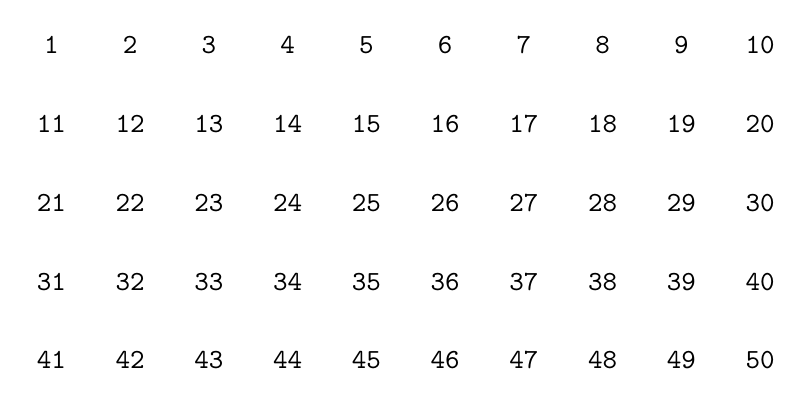
\begin{tikzpicture}
       \foreach \y in {0, 1, ..., 4}
       {
            \foreach \x in {1, 2, ..., 10}
            {
                \pgfmathtruncatemacro{\label}{(10*(4 - \y) + \x};
                \node at (\x, \y) { \tt \label };
            }
       }

    \end{tikzpicture}
    \end{figure}

\end{frame}

\begin{frame}[fragile]{Exemplo do crivo de Erastótenes para $N = 50$}

    \begin{figure}
    \centering
    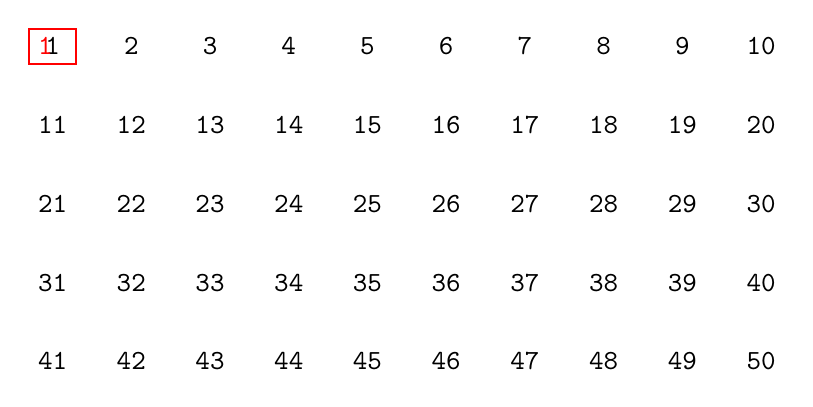
\begin{tikzpicture}
        \foreach \y in {0, 1, ..., 4}
        {
            \foreach \x in {1, 2, ..., 10}
            {
                \pgfmathtruncatemacro{\label}{(10*(4 - \y) + \x};
                \node at (\x, \y) { \tt \label };
            }
        }

        \foreach \n in { 1 }
        {
            \pgfmathtruncatemacro{\x}{\n - 10*round((\n - 1)/10)};
            \pgfmathtruncatemacro{\y}{4 - round((\n - 1)/10)};

            \node[draw, thick, red] at (\x, \y) {\tt \textcolor{red}{\n}};
        } 

    \end{tikzpicture}
    \end{figure}

\end{frame}

\begin{frame}[fragile]{Exemplo do crivo de Erastótenes para $N = 50$}

    \begin{figure}
    \centering
    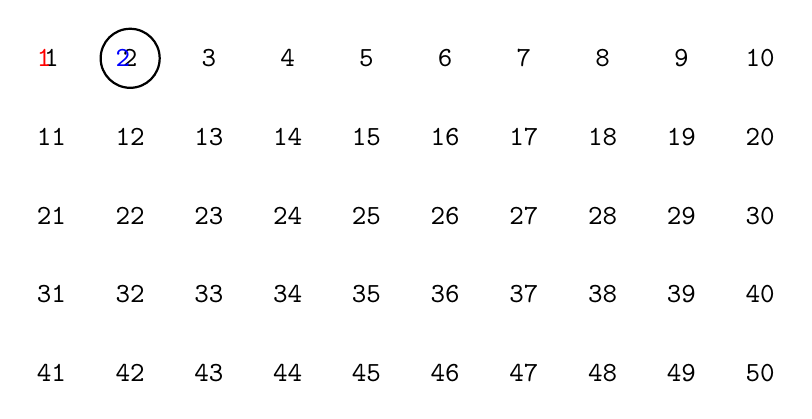
\begin{tikzpicture}
        \foreach \y in {0, 1, ..., 4}
        {
            \foreach \x in {1, 2, ..., 10}
            {
                \pgfmathtruncatemacro{\label}{(10*(4 - \y) + \x};
                \node at (\x, \y) { \tt \label };
            }
        }

        \foreach \n in { 1 }
        {
            \pgfmathtruncatemacro{\x}{\n - 10*round((\n - 1)/10)};
            \pgfmathtruncatemacro{\y}{4 - round((\n - 1)/10)};
            \node at (\x, \y) {\tt \textcolor{red}{\n}};
            %\node[draw, thick, red] at (\x, \y) {\tt \textcolor{red}{\n}};
        }

        \foreach \n in { 2 }
        {
            \pgfmathtruncatemacro{\x}{\n - 10*round((\n - 1)/10)};
            \pgfmathtruncatemacro{\y}{4 - round((\n - 1)/10)};
            \node[draw, circle, thick] at (\x, \y) {\tt \textcolor{blue}{\n}};
        }

    \end{tikzpicture}
    \end{figure}

\end{frame}

\begin{frame}[fragile]{Exemplo do crivo de Erastótenes para $N = 50$}

    \begin{figure}
    \centering
    \begin{tikzpicture}
        \foreach \y in {0, 1, ..., 4}
        {
            \foreach \x in {1, 2, ..., 10}
            {
                \pgfmathtruncatemacro{\label}{(10*(4 - \y) + \x};
                \node at (\x, \y) { \tt \label };
            }
        }

        \foreach \n in { 1 }
        {
            \pgfmathtruncatemacro{\x}{\n - 10*round((\n - 1)/10)};
            \pgfmathtruncatemacro{\y}{4 - round((\n - 1)/10)};
            \node at (\x, \y) {\tt \textcolor{red}{\n}};
        }

        \foreach \n in { 4, 6, ..., 50 }
        {
            \tikzmath{
                integer \k, \x;
                \k = (\n - 1)/10;
                \x = \n - 10*\k; 
                \y = 4 - \k; 
            }

            \node[draw, thick, red] at (\x, \y) {\tt \textcolor{red}{\n}};
        }

        \foreach \n in { 2 }
        {
            \pgfmathtruncatemacro{\x}{\n - 10*round((\n - 1)/10)};
            \pgfmathtruncatemacro{\y}{4 - round((\n - 1)/10)};
            \node[draw, circle, thick] at (\x, \y) {\tt \textcolor{blue}{\n}};
        }

    \end{tikzpicture}
    \end{figure}

\end{frame}

\begin{frame}[fragile]{Exemplo do crivo de Erastótenes para $N = 50$}

    \begin{figure}
    \centering
    \begin{tikzpicture}
        \foreach \y in {0, 1, ..., 4}
        {
            \foreach \x in {1, 2, ..., 10}
            {
                \pgfmathtruncatemacro{\label}{(10*(4 - \y) + \x};
                \node at (\x, \y) { \tt \label };
            }
        }

        \foreach \n in { 1 }
        {
            \pgfmathtruncatemacro{\x}{\n - 10*round((\n - 1)/10)};
            \pgfmathtruncatemacro{\y}{4 - round((\n - 1)/10)};
            \node at (\x, \y) {\tt \textcolor{red}{\n}};
        }

        \foreach \n in { 4, 6, ..., 50 }
        {
            \tikzmath{
                integer \k, \x;
                \k = (\n - 1)/10;
                \x = \n - 10*\k; 
                \y = 4 - \k; 
            }

            %\node[draw, thick, red] at (\x, \y) {\tt \textcolor{red}{\n}};
            \node at (\x, \y) {\tt \textcolor{red}{\n}};
        }

        \foreach \n in { 2, 3 }
        {
            \pgfmathtruncatemacro{\x}{\n - 10*round((\n - 1)/10)};
            \pgfmathtruncatemacro{\y}{4 - round((\n - 1)/10)};
            \node[draw, circle, thick] at (\x, \y) {\tt \textcolor{blue}{\n}};
        }

    \end{tikzpicture}
    \end{figure}

\end{frame}

\begin{frame}[fragile]{Exemplo do crivo de Erastótenes para $N = 50$}

    \begin{figure}
    \centering
    \begin{tikzpicture}
        \foreach \y in {0, 1, ..., 4}
        {
            \foreach \x in {1, 2, ..., 10}
            {
                \pgfmathtruncatemacro{\label}{(10*(4 - \y) + \x};
                \node at (\x, \y) { \tt \label };
            }
        }

        \foreach \n in { 1 }
        {
            \pgfmathtruncatemacro{\x}{\n - 10*round((\n - 1)/10)};
            \pgfmathtruncatemacro{\y}{4 - round((\n - 1)/10)};
            \node at (\x, \y) {\tt \textcolor{red}{\n}};
        }

        \foreach \n in { 4, 6, ..., 50 }
        {
            \tikzmath{
                integer \k, \x;
                \k = (\n - 1)/10;
                \x = \n - 10*\k; 
                \y = 4 - \k; 
            }

            \node at (\x, \y) {\tt \textcolor{red}{\n}};
        }

        \foreach \n in { 6, 9, ..., 50 }
        {
            \tikzmath{
                integer \k, \x;
                \k = (\n - 1)/10;
                \x = \n - 10*\k; 
                \y = 4 - \k; 
            }

            \node[draw, thick, red] at (\x, \y) {\tt \textcolor{red}{\n}};
        }


        \foreach \n in { 2, 3 }
        {
            \pgfmathtruncatemacro{\x}{\n - 10*round((\n - 1)/10)};
            \pgfmathtruncatemacro{\y}{4 - round((\n - 1)/10)};
            \node[draw, circle, thick] at (\x, \y) {\tt \textcolor{blue}{\n}};
        }

    \end{tikzpicture}
    \end{figure}

\end{frame}

\begin{frame}[fragile]{Exemplo do crivo de Erastótenes para $N = 50$}

    \begin{figure}
    \centering
    \begin{tikzpicture}
        \foreach \y in {0, 1, ..., 4}
        {
            \foreach \x in {1, 2, ..., 10}
            {
                \pgfmathtruncatemacro{\label}{(10*(4 - \y) + \x};
                \node at (\x, \y) { \tt \label };
            }
        }

        \foreach \n in { 1 }
        {
            \pgfmathtruncatemacro{\x}{\n - 10*round((\n - 1)/10)};
            \pgfmathtruncatemacro{\y}{4 - round((\n - 1)/10)};
            \node at (\x, \y) {\tt \textcolor{red}{\n}};
        }

        \foreach \n in { 4, 6, ..., 50 }
        {
            \tikzmath{
                integer \k, \x;
                \k = (\n - 1)/10;
                \x = \n - 10*\k; 
                \y = 4 - \k; 
            }

            \node at (\x, \y) {\tt \textcolor{red}{\n}};
        }

        \foreach \n in { 6, 9, ..., 50 }
        {
            \tikzmath{
                integer \k, \x;
                \k = (\n - 1)/10;
                \x = \n - 10*\k; 
                \y = 4 - \k; 
            }

            \node at (\x, \y) {\tt \textcolor{red}{\n}};
            %\node[draw, thick, red] at (\x, \y) {\tt \textcolor{red}{\n}};
        }


        \foreach \n in { 2, 3, 5 }
        {
            \pgfmathtruncatemacro{\x}{\n - 10*round((\n - 1)/10)};
            \pgfmathtruncatemacro{\y}{4 - round((\n - 1)/10)};
            \node[draw, circle, thick] at (\x, \y) {\tt \textcolor{blue}{\n}};
        }

    \end{tikzpicture}
    \end{figure}

\end{frame}

\begin{frame}[fragile]{Exemplo do crivo de Erastótenes para $N = 50$}

    \begin{figure}
    \centering
    \begin{tikzpicture}
        \foreach \y in {0, 1, ..., 4}
        {
            \foreach \x in {1, 2, ..., 10}
            {
                \pgfmathtruncatemacro{\label}{(10*(4 - \y) + \x};
                \node at (\x, \y) { \tt \label };
            }
        }

        \foreach \n in { 1 }
        {
            \pgfmathtruncatemacro{\x}{\n - 10*round((\n - 1)/10)};
            \pgfmathtruncatemacro{\y}{4 - round((\n - 1)/10)};
            \node at (\x, \y) {\tt \textcolor{red}{\n}};
        }

        \foreach \n in { 4, 6, ..., 50 }
        {
            \tikzmath{
                integer \k, \x;
                \k = (\n - 1)/10;
                \x = \n - 10*\k; 
                \y = 4 - \k; 
            }

            \node at (\x, \y) {\tt \textcolor{red}{\n}};
        }

        \foreach \n in { 6, 9, ..., 50 }
        {
            \tikzmath{
                integer \k, \x;
                \k = (\n - 1)/10;
                \x = \n - 10*\k; 
                \y = 4 - \k; 
            }

            \node at (\x, \y) {\tt \textcolor{red}{\n}};
        }

        \foreach \n in { 10, 15, ..., 50 }
        {
            \tikzmath{
                integer \k, \x;
                \k = (\n - 1)/10;
                \x = \n - 10*\k; 
                \y = 4 - \k; 
            }

            %\node at (\x, \y) {\tt \textcolor{red}{\n}};
            \node[draw, thick, red] at (\x, \y) {\tt \textcolor{red}{\n}};
        }


        \foreach \n in { 2, 3, 5 }
        {
            \pgfmathtruncatemacro{\x}{\n - 10*round((\n - 1)/10)};
            \pgfmathtruncatemacro{\y}{4 - round((\n - 1)/10)};
            \node[draw, circle, thick] at (\x, \y) {\tt \textcolor{blue}{\n}};
        }

    \end{tikzpicture}
    \end{figure}

\end{frame}

\begin{frame}[fragile]{Exemplo do crivo de Erastótenes para $N = 50$}

    \begin{figure}
    \centering
    \begin{tikzpicture}
        \foreach \y in {0, 1, ..., 4}
        {
            \foreach \x in {1, 2, ..., 10}
            {
                \pgfmathtruncatemacro{\label}{(10*(4 - \y) + \x};
                \node at (\x, \y) { \tt \label };
            }
        }

        \foreach \n in { 1 }
        {
            \pgfmathtruncatemacro{\x}{\n - 10*round((\n - 1)/10)};
            \pgfmathtruncatemacro{\y}{4 - round((\n - 1)/10)};
            \node at (\x, \y) {\tt \textcolor{red}{\n}};
        }

        \foreach \n in { 4, 6, ..., 50 }
        {
            \tikzmath{
                integer \k, \x;
                \k = (\n - 1)/10;
                \x = \n - 10*\k; 
                \y = 4 - \k; 
            }

            \node at (\x, \y) {\tt \textcolor{red}{\n}};
        }

        \foreach \n in { 6, 9, ..., 50 }
        {
            \tikzmath{
                integer \k, \x;
                \k = (\n - 1)/10;
                \x = \n - 10*\k; 
                \y = 4 - \k; 
            }

            \node at (\x, \y) {\tt \textcolor{red}{\n}};
        }

        \foreach \n in { 10, 15, ..., 50 }
        {
            \tikzmath{
                integer \k, \x;
                \k = (\n - 1)/10;
                \x = \n - 10*\k; 
                \y = 4 - \k; 
            }

            \node at (\x, \y) {\tt \textcolor{red}{\n}};
            %\node[draw, thick, red] at (\x, \y) {\tt \textcolor{red}{\n}};
        }


        \foreach \n in { 2, 3, 5, 7 }
        {
            \tikzmath{
                integer \k, \x;
                \k = (\n - 1)/10;
                \x = \n - 10*\k; 
                \y = 4 - \k; 
            }

            \node[draw, circle, thick] at (\x, \y) {\tt \textcolor{blue}{\n}};
        }

    \end{tikzpicture}
    \end{figure}

\end{frame}

\begin{frame}[fragile]{Exemplo do crivo de Erastótenes para $N = 50$}

    \begin{figure}
    \centering
    \begin{tikzpicture}
        \foreach \y in {0, 1, ..., 4}
        {
            \foreach \x in {1, 2, ..., 10}
            {
                \pgfmathtruncatemacro{\label}{(10*(4 - \y) + \x};
                \node at (\x, \y) { \tt \label };
            }
        }

        \foreach \n in { 1 }
        {
            \pgfmathtruncatemacro{\x}{\n - 10*round((\n - 1)/10)};
            \pgfmathtruncatemacro{\y}{4 - round((\n - 1)/10)};
            \node at (\x, \y) {\tt \textcolor{red}{\n}};
        }

        \foreach \n in { 4, 6, ..., 50 }
        {
            \tikzmath{
                integer \k, \x;
                \k = (\n - 1)/10;
                \x = \n - 10*\k; 
                \y = 4 - \k; 
            }

            \node at (\x, \y) {\tt \textcolor{red}{\n}};
        }

        \foreach \n in { 6, 9, ..., 50 }
        {
            \tikzmath{
                integer \k, \x;
                \k = (\n - 1)/10;
                \x = \n - 10*\k; 
                \y = 4 - \k; 
            }

            \node at (\x, \y) {\tt \textcolor{red}{\n}};
        }

        \foreach \n in { 10, 15, ..., 50 }
        {
            \tikzmath{
                integer \k, \x;
                \k = (\n - 1)/10;
                \x = \n - 10*\k; 
                \y = 4 - \k; 
            }

            \node at (\x, \y) {\tt \textcolor{red}{\n}};
            %\node[draw, thick, red] at (\x, \y) {\tt \textcolor{red}{\n}};
        }

        \foreach \n in { 14, 21, ..., 50 }
        {
            \tikzmath{
                integer \k, \x;
                \k = (\n - 1)/10;
                \x = \n - 10*\k; 
                \y = 4 - \k; 
            }

            \node[draw, thick, red] at (\x, \y) {\tt \textcolor{red}{\n}};
        }


        \foreach \n in { 2, 3, 5, 7 }
        {
            \tikzmath{
                integer \k, \x;
                \k = (\n - 1)/10;
                \x = \n - 10*\k; 
                \y = 4 - \k; 
            }

            \node[draw, circle, thick] at (\x, \y) {\tt \textcolor{blue}{\n}};
        }

    \end{tikzpicture}
    \end{figure}

\end{frame}


\begin{frame}[fragile]{Exemplo do crivo de Erastótenes para $N = 50$}

    \begin{itemize}
        \item Como o próximo número primo, a saber 11, é maior do que a raiz quadrada de 50, o 
            processo pode ser interrompido

        \item Os números não crivados formam a relação de todos os primos menores ou iguais a $N$

        \item Uma implementação do crivo de Erastótenes em C++ pode o vetor de \textit{bits} 
            \code{cpp}{sieve} para marcar os números

        \item Zero ou falso indica que o número não é primo
    \end{itemize}

\end{frame}

\begin{frame}[fragile]{Implementação do crivo em C++}
    \inputsnippet{cpp}{66}{82}{codes/primes.cpp}
\end{frame}

\begin{frame}[fragile]{Aproximação para a complexidade do crivo}

    \begin{itemize}
        \item Na rotina \code{cpp}{primes2()}, para cada $i$ são crivados $N/i$ números

        \item Portanto o número total $T(N)$ de operações é aproximadamente $N$ vezes o $N$-ésimo 
            número harmônico $H_N$, isto é,
$$
   T(N) \approx N + \frac{N}{2} + \frac{N}{3} + \ldots + \frac{N}{N} = N\times H_N =  N\left(1 + \frac{1}{2} + \frac{1}{3} + \ldots + \frac{1}{N}\right) \leq N \log N
$$

        \item A desigualdade vale porque 
$$
    \log N = \int_1^N \frac{1}{x} dx \geq \sum_{i = 1}^N  \frac{1}{i}
$$
    \end{itemize}

\end{frame}

\begin{frame}[fragile]{Complexidade do Crivo de Erastótenes}

    \begin{itemize}
        \item Na aproximação para $T(N)$ a variável $i$ assume todos os naturais no intervalo 
            $[1, N]$, inclusive números compostos

        \item Porém na implementação $i$ assume apenas valores primos

        \item Uma melhor aproximação seria, pelo Teorema de Merten,
$$
\frac{N}{2} + \frac{N}{3} + \frac{N}{5} + \frac{N}{7} + \frac{N}{11} + \ldots \leq N\log\log N
$$

        \item Logo a complexidade do crivo é $O(N\log \log N)$
    \end{itemize}

\end{frame}

\begin{frame}[fragile]{Redução da constante de complexidade}

    \begin{itemize}
        \item A implementação de \code{cpp}{primes2()} é simples e direta

        \item É possível, contudo, diminuir a constante de complexidade e obter um melhor tempo de
            execução

        \item Primeiramente, os números pares podem ser tratados à parte: 2 é o único primo par, e
            os demais pares compostos não contribuem para o crivo

        \item O número 1 pode ser desprezado, uma vez que a saída da rotina é uma lista de primos

    \end{itemize}

\end{frame}

\begin{frame}[fragile]{Crivo com tratamento diferente para pares}
    \inputsnippet{cpp}{84}{100}{codes/primes.cpp}
\end{frame}

\begin{frame}[fragile]{Nova redução da constante de complexidade}

    \begin{itemize}
        \item Embora o laço externo de \code{cpp}{primes3()} só considere números ímpares, o laço 
            interno itera por pares desnecessariamente

        \item Outra observação importante: o crivo deve começar no quadrado de $i$, pois quaisquer
            múltiplos de $i$ menores do que $i^2$ já foram crivados

        \item Estas duas observações reduzem novamente a constante de complexidade 

        \item Para evitar problemas de \textit{overflow} na condição do laço interno, o tipo de
            dado foi alterado de \code{cpp}{int} para \code{cpp}{long long}
    \end{itemize}

\end{frame}

\begin{frame}[fragile]{Crivo sem pares nos laços}
    \inputsnippet{cpp}{102}{118}{codes/primes.cpp}
\end{frame}

\begin{frame}[fragile]{Tratamento de múltiplos de 3 à parte}

    \begin{itemize}
        \item Assim como foi feito para os pares, os múltiplos de 3 também podem ser tratados à 
            parte

        \item A inclusão prévia do 3 na lista de primos é a parte trivial: difícil é evitar os 
            múltiplos de 3 no laço externo

        \item Isto pode ser feito observando que, seguindo a sequência dos ímpares a partir de 3, 
            primeiro há um múltiplo de 3, depois um número cujo resto da divisão por 3 é 2, por
            fim um número cuja divisão por 3 é 1, e o ciclo se reinicia

        \item Os múltiplos de 3, portanto, podem ser ignorados


    \end{itemize}

\end{frame}

\begin{frame}[fragile]{Crivo com múltiplos de $2$ e $3$ tratados à parte}
    \inputsnippet{cpp}{120}{136}{codes/primes.cpp}
\end{frame}

\begin{frame}[fragile]{Verificação das implementações do crivo}

Uma maneira de verificar rapidamente se o crivo está produzindo os primos corretamente é checar o
número de primos gerados, segundo a tabela abaixo:

\begin{table}[!h]
    \centering
    \begin{tabular}{lr}
        \toprule
        $n$ & $\pi(n)$\\
        \midrule
        10 & 4 \\
        100 & 25 \\
        1000 & 168 \\
        10000 & 1229 \\
        100000 & 9592 \\
        1000000 & 78498 \\
        10000000 & 664579 \\
        \bottomrule
    \end{tabular}
\end{table}

\end{frame}

\begin{frame}[fragile]{Possível saída para as rotinas de teste de primalidade}
    \begin{footnotesize}
    \begin{verbatim}
    ==== Testes de primalidade:

    is_prime(999983)  = 1 (0.010074394000000 ms)
    is_prime2(999983) = 1 (0.005721907000000 ms)
    is_prime3(999983) = 1 (0.000006486000000 ms)


    ==== Geração de primos até N:

    primes(10000000)  = 664579 (2.428975496000000 ms)
    primes2(10000000) = 664579 (0.172493493000000 ms)
    primes3(10000000) = 664579 (0.136014180000000 ms)
    primes4(10000000) = 664579 (0.067260405000000 ms)
    primes5(10000000) = 664579 (0.059135050000000 ms)
    \end{verbatim}
    \end{footnotesize}
\end{frame}

\begin{frame}[fragile]{Problemas propostos}

    \begin{enumerate}
        \item \href{https://atcoder.jp/contests/abc096/tasks/abc096_d}{AtCoder Beginner Contest 096D -- Five, Five Everywhere}
        \item \href{https://atcoder.jp/contests/abc149/tasks/abc149_c}{AtCoder Beginner Contest 149C -- Next Prime}
        \item \href{https://codeforces.com/problemset/problem/327/B}{Codeforces 327B -- Hungry Sequence}
        \item \href{http://onlinejudge.org/index.php?option=com_onlinejudge&Itemid=8&category=24&page=show_problem&problem=484}{OJ 543 -- Goldbach}
        \item \href{http://uva.onlinejudge.org/index.php?option=com_onlinejudge&Itemid=8&category=24&page=show_problem&problem=1942}{OJ 11001 -- Necklace}
    \end{enumerate}

\end{frame}
